\documentclass[a4paper,12pt]{article}
\usepackage[left=2.5cm, right=2.5cm, top=3cm, bottom=3cm]{geometry}
\usepackage[spanish]{babel}
\usepackage{graphicx}
\usepackage[utf8]{inputenc}
  
\begin{document}
\title{Primer Proyecto de Programación}
\author{Barbaro Yoel Martinez Gonzalez C113}
\date{2023}
\maketitle



 \begin{abstract}
 Moogle!:es una aplicación web *totalmente original* cuyo propósito es buscar inteligentemente un texto en un conjunto
de documentos.desarrollada con tecnología .NET Core 7.0,específicamente usando Blazor como *framework* web para la interfaz
gráfica, y en el lenguaje C$\#$.
\end{abstract}

\begin{figure}[h]
	\center
	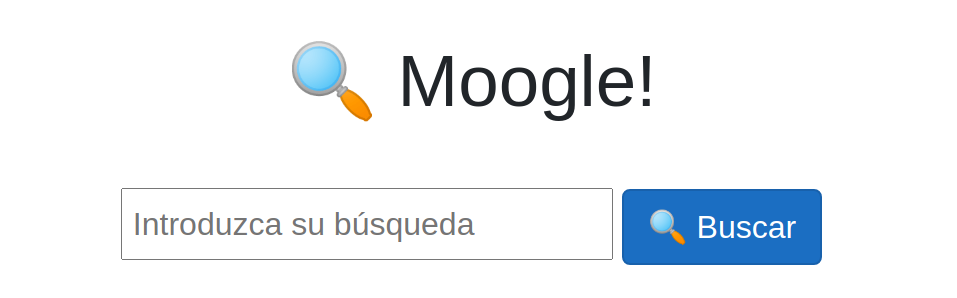
\includegraphics[width=8cm]{moogle.png}
	\caption{Moogle!}
	\label{fig:logo}
\end{figure}
%Proyecto de Programación I.
%Facultad de Matemática y Computación - Universidad de La Habana.
%Cursos 2021, 2022, 2023.


\section{Flujo de Funcionamiento}

En este proyecto se han empleado varias clases, las cuales al combinarlas crearían un buen funcionamiento del moogle.

Class Folder recibe en su constructor la ruta del directorio que contiene a los archivos. Este mismo string es asignado al estring folder, de la ruta se podían obtener las rutas de los archivos q estén dentro de esa carpeta, es por eso q creamos un array de string llamado *filesroot* y guardamos en este archivo array las rutas de los archivos q estan dentro de la carpeta content. Encontramos también un entero de nombre *numberOfFiles* q va a contar los elementos del array mencionado anteriormente. 

También creamos una *classFile*(clase archivo) q tiene   como propiedades el nombre de un archivo *fileName*, el contenido de un archivo *content* y la ruta del archivo *fileRoute*, todos salen de la ruta de la carpeta inicial *folder*. Está la propiedad de guardar las palabras del contenido del archivo en un array al cual le llamaremos *wordsInArray*. El filename se obtiene a través de un método llamado GetFileName() el cual tiene como parámetro la ruta del archivo. Content será encontrado por el método GetFileContent() Al cual también c le pasará como parámetro la ruta del archivo. Para wordsInArray se debe crear otra clase llamada classTokenize la cual tendrá varios metodos, uno de ellos se llamará StringToArray y llevará el contenido a minúsculas, y con Using System.Text y Using system.Text.RegularExpresions declarados podemos utilizar la clase Regex para sustituir los caracteres extraños por espacios en blanco q serían eliminados en otro método de la misma clase llamado StrangeCharacterRemover y las palabras serían guardadas en un array

En la zona del TF-IDF tenemos el TF determinado en classFile y hayado mediante el método WordsCounter q recibe como parámetro wordsInArray y por cada palabra de este array va a contar cuantas veces aparece y devolverlo como diccionario q tiene como keys las palabras de wordsInArray y como value la cantidad de veces q aparece. El IDF  lo hallaremos mediante un método pasando como parámetro el string word; este idf retornará como un valor float y la fórmula aplicada a este va a contener el entero numberOfFiles un método al q le llamamos GetNumberOfAppearences q recibe como parámetro un string word, este método nos da las apariciones de una palabra en la carpeta. Para esto se creó un diccionario en la classFolder llamado AllTFs q tendrá como keys un string q será el nombre del archivo y su value será otro diccionario q tendrá las palabras de los archivos y cuantas veces aparecen

El otro .cs tenego la classQuery(clase query) la cual tiene como propiedad el contenido de la query en un string llamado QueryContent, tiene también un array de string llamado QueryContentInArray el cual hallamos mediante un método de la clase tokenize, el método llamado StringToArray y le pasaremos como parámetro el QueryContent mencionado anteriormente; recibiremos las palabras de la query en un array. Otra propiedad es el diccionario QueryRelevance q posee como Keys las palabras de wordsInArray y como value la cantidad de veces q se repiten, a los values de este diccionario los dividiremos entre la extensión de wordsInArray y luego lo multiplicaremos por el idf de la palabra

La clase Engine es la que contiene el método principal de búsqueda Searcher, que recibe la carpeta de base de datos (DataBase) y la cadena de consulta de búsqueda (InputQuery).
La función Searcher comienza creando una nueva instancia de la clase Query con la cadena de consulta proporcionada y almacena la sugerencia de búsqueda (suggestion) que es inicializada con el mismo valor de la cadena de consulta.
Luego, se accede a la matriz de relevancia (Relevance) dentro de la base de datos (DataBase.Relevance), que parece ser una matriz de diccionarios anidados.Kevin, [25/7/23 21:48]
Se crea una lista vacía de objetos SearchItem (items) para almacenar los resultados de búsqueda.
A continuación, se recorren los archivos dentro de la base de datos (DataBase.Files) y se realiza el siguiente proceso:
Se obtiene el título del archivo (title) y se obtiene un fragmento del contenido del archivo relacionado con la consulta utilizando el método privado GetSnippet.
Se calcula una puntuación (score) para el archivo en función de la consulta y la matriz de relevancia usando el método privado GetScore.
Se crea un objeto SearchItem con el título, el fragmento y la puntuación, y se agrega a la lista de resultados (items) si el fragmento no es nulo.
Luego, los elementos en la lista de resultados (items) se ordenan en orden descendente según su puntuación.
Finalmente, se crea un nuevo arreglo de SearchItem (finalItems) a partir de la lista ordenada y se crea un objeto SearchResult con estos resultados y la sugerencia de búsqueda original, que es lo que se devuelve.
Métodos privados GetScore y GetSnippet:
GetScore es un método privado que calcula la puntuación de relevancia de un archivo específico para una consulta dada. Utiliza una técnica que parece implicar un cálculo de similitud de coseno entre la consulta y el contenido del archivo en función de una matriz de relevancia precalculada.
GetSnippet es otro método privado que devuelve un fragmento del contenido del archivo con la consulta resaltada en negrita. El fragmento incluye 50 caracteres antes y después de la primera aparición de la consulta en el contenido del archivo.
Otros métodos privados WordsImportance y Partition:
WordsImportance filtra una lista de palabras (representada por un array de strings) y devuelve solo las palabras que cumplen ciertos criterios relacionados con la existencia de las palabras en la base de datos y su longitud.
Partition toma una matriz de palabras y devuelve una submatriz basada en los índices de inicio y fin proporcionados.

En la clase "Moogle", hay una variable estática llamada "DataBase" que se utiliza para almacenar la carpeta de datos del motor de búsqueda. También hay una variable estática booleana llamada "Initied" que indica si el motor de búsqueda ha sido inicializado.
La primera función es "Query", que toma una cadena de consulta como parámetro y devuelve un resultado de búsqueda. Antes de hacer cualquier búsqueda, primero se llama a la función "Init" para asegurarse de que el motor de búsqueda esté inicializado.
Dentro de la función "Query", hay una serie de condicionales para manejar diferentes situaciones. Si la consulta no está vacía y la ruta de archivos de la base de datos no es nula, se realiza una búsqueda utilizando el método "Searcher" de una clase "Engine" y se devuelve el resultado.
Si la consulta está vacía, se crea un objeto de tipo "SearchItem" con un mensaje indicando al usuario que ingrese una palabra o frase para realizar una búsqueda. Luego, se crea un array que contiene ese único "SearchItem" y se devuelve un "SearchResult" que contiene este array.
Si la consulta no está vacía y la ruta de archivos de la base de datos es nula , simplemente se devuelve un "SearchResult" vacío.
A continuación, tenemos la función "Init", que se encarga de inicializar la base de datos si aún no ha sido inicializada. Si "Initied" es falso, crea una nueva instancia de "Folder" y establece "Initied" en verdadero para indicar que la inicialización se ha realizado.

\section{Correr el proyecto y la busqueda }
Para correr el proyecto debes usar el comando dotnet watch run --project MoogleServer en Windows y make dev en Linux. En la carpeta Content deberán aparecer los documentos
(en formato *.txt)en los que el usuario va a realizar la búsqueda. En la casilla donde aparece Introduzca la búsqueda el usuario va a escribir que desea buscar y basta con apretar el botón Buscar para que Moogle! haga su trabajo.

\newpage
\section{Fuentes que utilicé:}
\begin{itemize}
	\item Wikipedia
	\item Github
    \item ChatGpt

\end{itemize}


\end{document}
